\documentclass[12pt,a4paper]{article}
\usepackage[utf8]{inputenc}
\usepackage[T1]{fontenc}
\usepackage[polish]{babel}
\usepackage{float}
\usepackage{cite}

\usepackage{pgfplots}
\usepackage{pgfplotstable}
\pgfplotsset{compat=newest}

\begin{document}

\title{[PSZT] PZ.U17 - Marketing bankowy}
\author{Adrian Brodzik \and Jakub Górka}
\maketitle

\section*{Zadanie}
Porównać algorytmy regresji logistycznej i XGBoost.

\section*{Teza}
\textbf{Efektywność regresji logistycznej i XGBoost jest równa dla problemu ustalenia potencjalnych klientów lokat bankowych pewnej portugalskiej instytucji finansowej.}

\section*{Analiza danych}
Źródło danych: \texttt{https://archive.ics.uci.edu/ml/datasets/Bank+Marketing}
\\
Plik danych: \texttt{bank-additional-full.csv}
\\
Opis danych: \texttt{bank-additional-names.txt}
\\
\\
Zbiór danych wykorzystywanych w projekcie pochodzi z kampanii marketingowej lokaty terminowej
prowadzonej przez portugalską instytucję finansową. Owa kampania oparta była o kontakt
telefoniczny. Każdy rekord przedstawia jednego klienta, z podziałem na poszczególne atrybuty.
\\
\\
Atrybuty wejściowe przedstawiają szczegóły danego klienta umożliwiające dokładniejszą klasyfikację,
natomiast atrybutem wyjściowym jest informacja o decyzji przystąpieniu do lokaty terminowej.
Podział względem poszczególnych atrybutów, pozwala stwierdzić iż dominującą grupą wiekową są
osoby w wieku 31-40, niestety nie wiemy nic o podziale na płeć poszczególnych osób. Kolejną
obserwacją jest większościowy udział osób po ślubie. Dominującym zawodem wśród klientów były
osoby administracji publicznej. Pod względem wykształcenia osoby które najczęściej decydowały się
na lokatę były osobami, które uzyskały wykształcenie podstawowe oraz uniwersyteckie. Atrybut
\textit{duration} nie jest uwzględniany w analizie i nie jest używany w doświadczeniu tworzenia modelu
predykcyjnego ze względu na niewiedzę zakończenia trwającej rozmowy.

\begin{figure}[H]
	\centering
	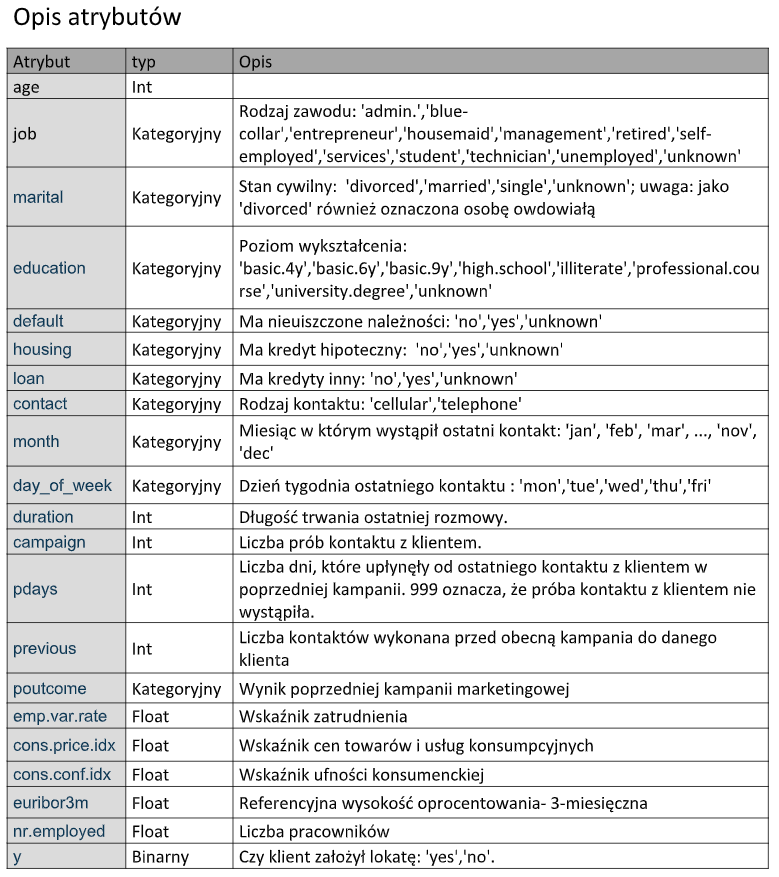
\includegraphics[scale=0.65]{data_1.png}
\end{figure}

\begin{figure}[H]
	\centering
	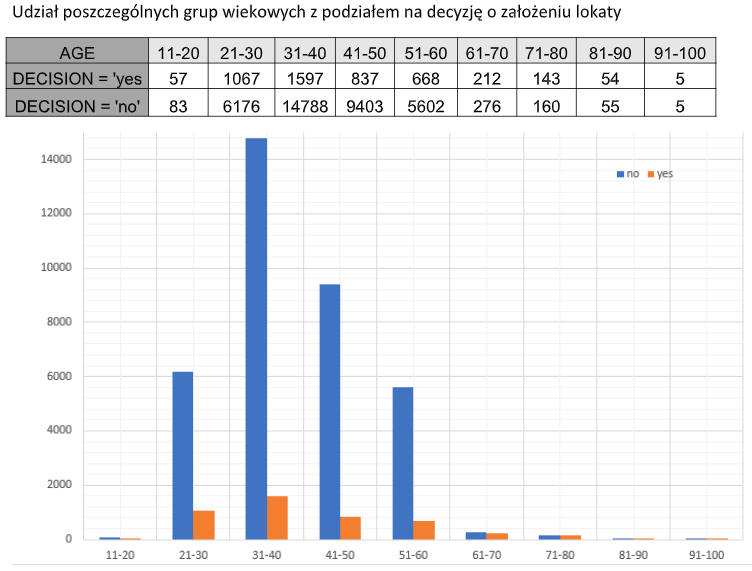
\includegraphics[scale=0.65]{data_2.png}
\end{figure}

\begin{figure}[H]
	\centering
	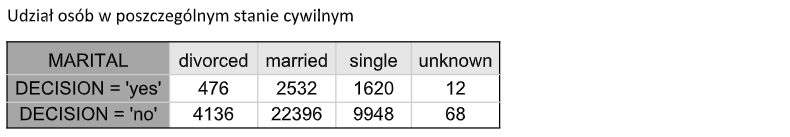
\includegraphics[scale=0.65]{data_3.png}
\end{figure}

\begin{figure}[H]
	\centering
	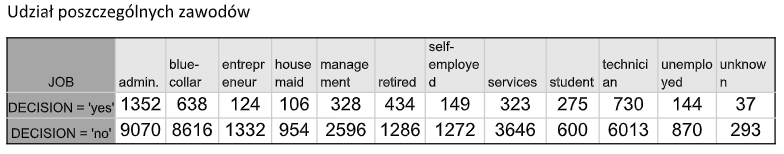
\includegraphics[scale=0.65]{data_4.png}
\end{figure}

\begin{figure}[H]
	\centering
	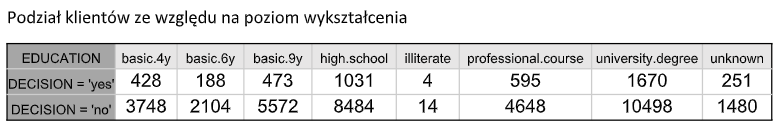
\includegraphics[scale=0.65]{data_5.png}
\end{figure}

\begin{figure}[H]
	\centering
	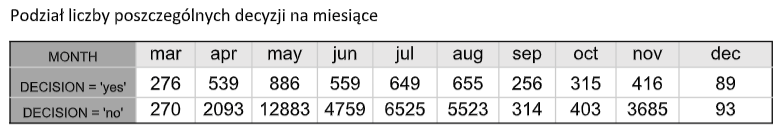
\includegraphics[scale=0.65]{data_6.png}
\end{figure}

\begin{figure}[H]
	\centering
	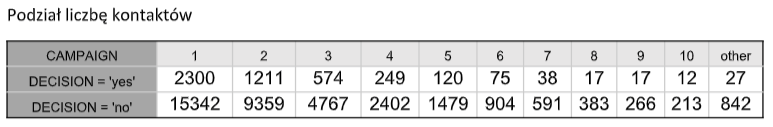
\includegraphics[scale=0.65]{data_7.png}
\end{figure}

\section*{Eksperyment}
Dane są ładowane z pliku \texttt{bank-additional-full.csv} do pamięci za pomocą modułu \texttt{pandas}.
\\
\\
Wartości kolumny celu \textit{y} są mapowane na $0$ dla wartości \textit{no}, albo $1$ dla wartości \textit{yes}. Następnie wartości kolumn kategorycznych są jednoznacznie mapowane na liczby całkowite dodatnie. Gdyby model był zapisany i uruchomiony na nowych danych, to wartości danych powinny być dokładnie tak zakodowane, jak podczas procesu uczenia się modelu. Natomiast dane, które nigdy wcześniej się nie pojawiły, są kodowane na wartość wyrażenia \texttt{\_\_UNKNOWN\_\_}. Na koniec usuwane są kolumny niepotrzebne (w zależności od wykonywanego eksperymentu).
\\
\\
Do podziału danych wykorzystany jest proces k-krotnej walidacji z modułu \texttt{scikit-learn}. Ponadto dane są rozłożone równomiernie ze względu na wartość kolumny celu \textit{y} (ang. \textit{stratified k-fold}).
\\
\\
W każdej z $k$ iteracji generowane są dwa zbiory danych: treningowy oraz walidacyjny. Zbiór treningowy służy do uczenia modelu \texttt{LogisticRegression} z modułu \texttt{scikit-learn} albo \texttt{XGBRegressor} z modułu \texttt{XGBoost}. Zbiór walidacyjny służy do oceny nauczonego modelu, np. za pomocą \texttt{roc\_auc\_score} z modułu \texttt{scikit-learn}. ROC-AUC określa w jakim stopniu nauczony model jest w stanie rozpoznać daną klasę.

\section*{Hiperparametry}
Do automatycznego strojenia parametrów wykorzystano moduł \texttt{hyperopt}, a w szczególności estymator jądrowy gęstości (ang. \textit{Tree-structured Parzen Estimator}).
\\
\\
Dla regresji logistycznej przeszukano następujące parametry:
\begin{itemize}
	\item tol - tolerancja błędu, aby doszło do wczesnego zatrzymania
	\item C - odwrotność siły regularyzacji
	\item fit\_intercept - czy powinna być dodana stała, np. bias
	\item class\_weight - wagi klas
	\item solver - algorytm optymalizacyjny
	\item max\_iter - maksymalna liczba iteracji
\end{itemize}
Dla XGBoost przeszukano następujące parametry:
\begin{itemize}
	\item n\_estimators - liczba drzew
	\item max\_depth - maksymalna głębokość drzew
	\item learning\_rate - współczynnik nauczania
	\item booster - algorytm wzmocnienia gradientowego
	\item tree\_method - algorytm konstruowania drzew
	\item gamma - minimalna redukcja błędu potrzebna, aby doszło do podziału liścia
	\item subsample - współczynnik instancji treningowej
	\item colsample\_bytree - współczynnik kolumn podczas budowania drzewa
	\item colsample\_bylevel - współczynnik kolumn dla każdego poziomu w drzewie
	\item colsample\_bynode - współczynnik kolumn do podziału
	\item reg\_alpha - regularyzacja L1
	\item reg\_lambda - regularyzacja L2
	\item scale\_pos\_weight - równoważenie dodatnich i ujemnych wag
\end{itemize}

\pgfplotstableread{
	X	Y
	2	78.69714909632302
	3	78.66706102134483
	4	78.67094831360176
	5	78.65894483912202
	6	78.67538476795796
	7	78.63251478833636
	8	78.67570483656661
	9	78.68297518084827
	10	78.66307845322866
	11	78.6612037183697
	12	78.67152659420497
	13	78.69409588069043
	14	78.66424887897095
	15	78.67461243178607
}\datatableA

\pgfplotstableread{
	X	Y
	2	80.45327377695086
	3	80.44886331500206
	4	80.58865903318451
	5	80.47481124606423
	6	80.71345737170446
	7	80.57273195610956
	8	80.60197838197677
	9	80.75462585435221
	10	80.6557763109069
	12	80.67750282856588
	15	80.67771125986073
}\datatableB

\section*{Wyniki}
\begin{figure}[H]
	\centering
	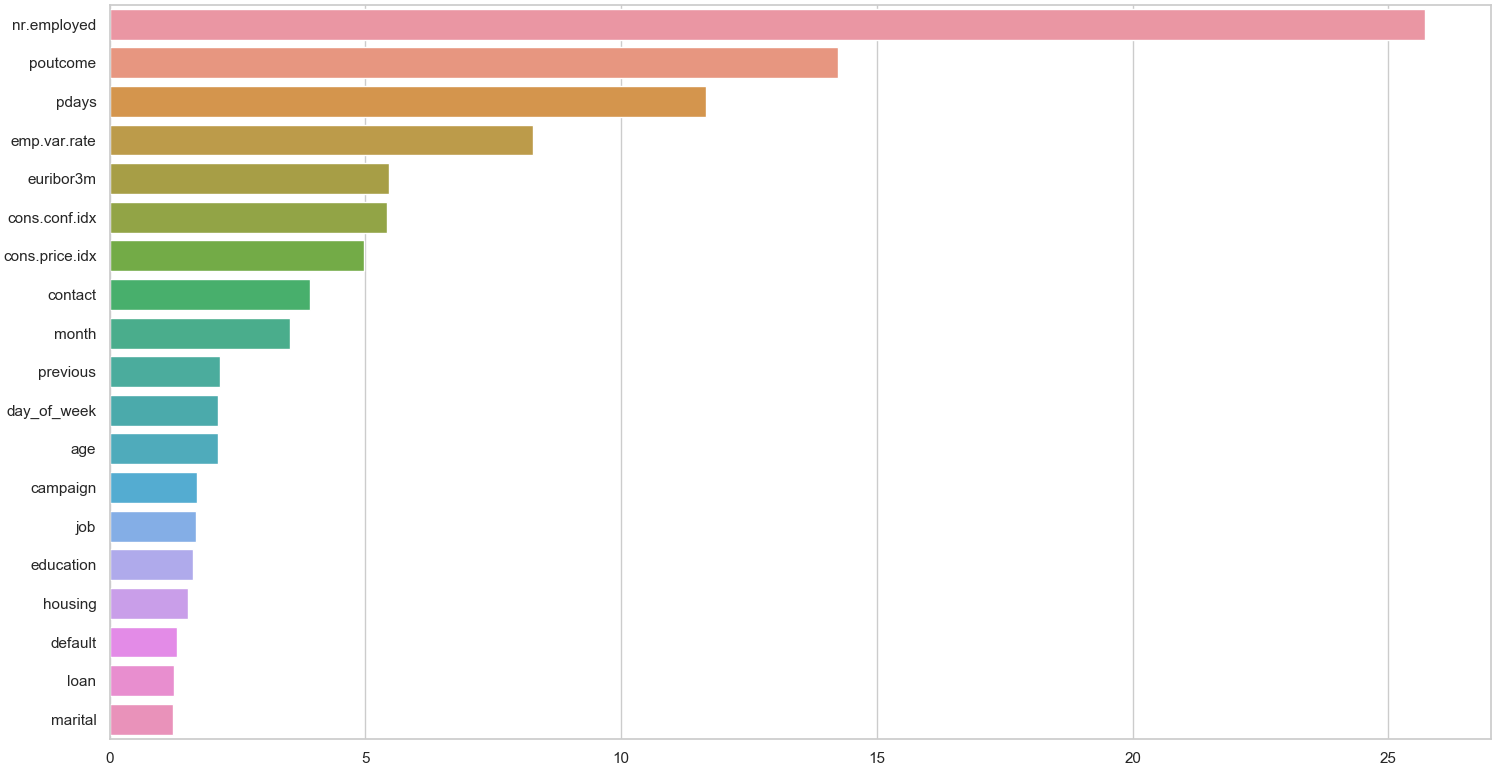
\includegraphics[scale=0.35]{features.png}
	\caption{\textbf{Najważniejsze kolumny wg XGBoost} (bez \textit{duration})}
\end{figure}

\begin{figure}[H]
	\centering
	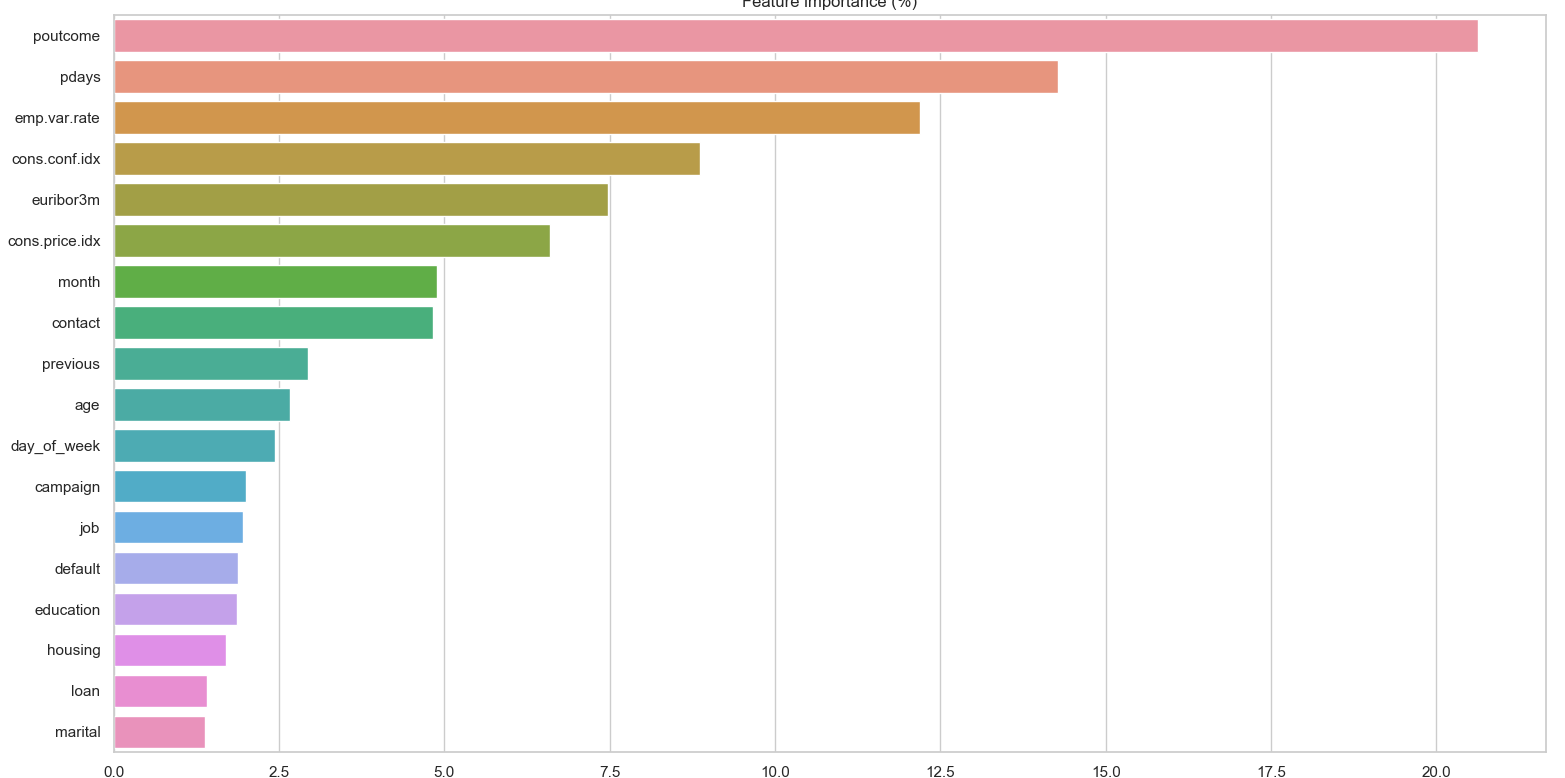
\includegraphics[scale=0.35]{features_2.png}
	\caption{\textbf{Najważniejsze kolumny wg XGBoost} (bez \textit{duration}, \textit{nr.employed})}
\end{figure}

\begin{table}[H]
	\centering
	\begin{tabular}{c|c|c}
		seed & \begin{tabular}[c]{@{}c@{}}regresja logistyczna\\ ROC AUC (\%)\end{tabular} & \begin{tabular}[c]{@{}c@{}}XGBoost\\ ROC AUC (\%)\end{tabular} \\ \hline
		42 & 78.60 & 80.54 \\ \hline
		64 & 78.63 & 80.50 \\ \hline
		100 & 78.69 & 80.70 \\ \hline
		123 & 78.65 & 80.47 \\ \hline
		234 & 78.63 & 80.48 \\ \hline
		345 & 78.63 & 80.65 \\ \hline
		456 & 78.59 & 80.53 \\ \hline
		567 & 78.56 & 80.53 \\ \hline
		678 & 78.69 & 80.60 \\ \hline
		789 & 78.69 & 80.60
	\end{tabular}
	\caption{Wyniki (bez kolumny \textit{duration})}
\end{table}

\begin{table}[H]
	\centering
	\begin{tabular}{c|c|c}
		seed & \begin{tabular}[c]{@{}c@{}}regresja logistyczna\\ ROC AUC (\%)\end{tabular} & \begin{tabular}[c]{@{}c@{}}XGBoost\\ ROC AUC (\%)\end{tabular} \\ \hline
		42 & 93.23 & 95.07 \\ \hline
		64 & 93.24 & 95.00 \\ \hline
		100 & 93.24 & 95.07 \\ \hline
		123 & 93.23 & 95.06 \\ \hline
		234 & 93.23 & 95.05 \\ \hline
		345 & 93.21 & 95.03 \\ \hline
		456 & 93.24 & 95.05 \\ \hline
		567 & 93.23 & 94.99 \\ \hline
		678 & 93.23 & 95.01 \\ \hline
		789 & 93.23 & 95.09
	\end{tabular}
	\caption{Wyniki (wszystkie kolumny)}
\end{table}

\begin{figure}[H]
	\centering
	\begin{tikzpicture}
	\begin{axis}[
		xlabel=k,
		ylabel=ROC AUC (\%),
		grid=both,
		xmin=2,
		ymin=78.63,
		xmax=15,
		ymax=78.7,
		scale=1.5
	]
	\addplot [only marks, red] table {\datatableA};
	\end{axis}
	\end{tikzpicture}
	\caption{\textbf{Regresja logistyczna i k-krotna walidacja.} Wyższa ocena świadczy o efektywniejszej klasyfikacji.}
\end{figure}

\begin{figure}[H]
	\centering
	\begin{tikzpicture}
	\begin{axis}[
		xlabel=k,
		ylabel=ROC AUC (\%),
		grid=both,
		xmin=2,
		ymin=80.4,
		xmax=15,
		ymax=80.7,
		scale=1.5
	]
	\addplot [only marks, blue] table {\datatableB};
	\end{axis}
	\end{tikzpicture}
	\caption{\textbf{XGBoost i k-krotna walidacja.} Wyższa ocena świadczy o efektywniejszej klasyfikacji.}
\end{figure}

\section*{Dyskusja}
W przypadku użycia wszystkich kolumn oba algorytmy otrzymały wyższe wyniki. Stało się tak, ponieważ kolumna \textit{duration} ma duży wpływ na kolumnę docelową \textit{y}. W pozostałych testach nie użyto \textit{duration}.
\\
\\
Usunięcie kolumny \textit{nr.employed} nie wpłynęło negatywnie na efektywność modeli mimo tego, że była to najważniejsza kolumna według XGBoost. Najważniejszą kolumną stała się wówczas \textit{poutcome}, tzn. obecny wynik głównie zależy od wyniku poprzedniej rozmowy z klientem. Ponadto ważne są kolumny dotyczące koniunktury rynku, np. \textit{euribor3m}.
\\
\\
Wyższa wartość $k$ w procesie k-krotnej walidacji nie oznacza, że klasyfikator będzie efektywniejszy. Zbiór treningowy jest proporcjonalnie większy, ale zbiór walidacyjny jest proporcjonalnie mniejszy. Ciężko jest wykryć przeuczenie modelu, mając zbyt mały zbiór walidacyjny.

\section*{Wnioski}
Teza została potwierdzona w granicy błędu $2\%-3\%$ ROC AUC. Regresja logistyczna i XGBoost są skutecznymi algorytmami do klasyfikacji obiektów z zadanej przestrzeni i detekcji nieliniowych relacji między nimi.
\\
\\
XGBoost osiągnął lepszy wynik, ale jego złożoność i czas obliczeniowy był znacznie gorszy w porównaniu do prostszego algorytmu regresji logistycznej. Model regresji logistycznej, który właściwie jest uogólnionym modelem liniowym, jest prostszy w konstrukcji i zrozumieniu niż losowo generowane drzewa decyzyjne XGBoost. Dlatego też większość instytucji finansowych preferuje, albo nawet musi, używać tych prostszych modeli.
\\
\\
XGBoost i podobne biblioteki wzmocnień gradientowych mają szerokie zastosowanie w bardziej skomplikowanych problemach, w szczególności konkursach sztucznej inteligencji, gdzie oprócz strojenia parametrów, konieczna jest inżyniera danych.

\nocite{*}
\bibliographystyle{plain}
\bibliography{Raport}{}

\end{document}